%\documentclass[aspectratio=43]{beamer}
%\documentclass[aspectratio=1610]{beamer}
\documentclass[aspectratio=169]{beamer}

% @IMP@ \usepackage{pgfpages}
% @IMP@ \pgfpagesuselayout{2 on 1}[a4paper,border shrink=5mm]

\usepackage{fixltx2e}

\usepackage[english,french]{babel}
\usepackage[T1]{fontenc}
\usepackage[utf8]{inputenc}
\usepackage{microtype}

\usepackage{lmodern}

\usepackage{amsmath}
\usepackage{array}
\usepackage{bookmark}
\usepackage{graphicx}
\usepackage{keystroke}
\usepackage{marvosym}
\usepackage{siunitx}
\usepackage{tabularx}
\usepackage{tabulary}
\usepackage{tikz}
\usepackage{xspace}

\usepackage{formation}

% beamer

%\usetheme[formation]{Linagora}
\usetheme{metropolis}

\title{PostgreSQL}
\subtitle{DBA Infrastructure}

%\setbeameroption{show notes}

% array

\setlength{\extrarowheight}{2pt}

% babel

\frenchbsetup{og=«,fg=»}

\newcommand{\anglais}[1]{\textit{\foreignlanguage{english}{#1}}}

% graphicx

\graphicspath{{illustrations/}}

% marvosym

\newcommand{\curseur}{\Rectsteel}

% siunitx

\sisetup
{
	binary-units	= true ,
}

\DeclareSIUnit{\octet}{o}

% tikz

\usetikzlibrary{calc,decorations.pathmorphing}

%%%%%%%%%%%%%%%%%%%%%%%%%%%%%%%%%%%%%%%%%%%%%%%%%%%%%%%%%%%%%%%%%%%%%%%%%%%%%%%%

\begin{document}

%%%%%%%%%%%%%%%%%%%%%%%%%%%%%%%%%%%%%%%%%%%%%%%%%%%%%%%%%%%%%%%%%%%%%%%%%%%%%%%%

\begin{frame}

\pdfbookmark[2]{\inserttitle\ -- \insertsubtitle}{titre}

\titlepage

\end{frame}

%%%%%%%%%%%%%%%%%%%%%%%%%%%%%%%%%%%%%%%%%%%%%%%%%%%%%%%%%%%%%%%%%%%%%%%%%%%%%%%%

\section*{Introduction}

\pdfbookmark[2]{Introduction}{introduction}

%%%%%%%%%%%%%%%%%%%%%%%%%%%%%%%%%%%%%%%%%%%%%%%%%%%%%%%%%%%%%%%%%%%%%%%%%%%%%%%%

\section{PostgreSQL Internals}

%%%%%%%%%%%%%%%%%%%%%%%%%%%%%%%%%%%%%%%%%%%%%%%%%%%%%%%%%%%%%%%%%%%%%%%%%%%%%%%%

\subsection{Point in Time Recovery}

%%%%%%%%%%%%%%%%%%%%%%%%%%%%%%%%%%%%%%%%%%%%%%%%%%%%%%%%%%%%%%%%%%%%%%%%%%%%%%%%

\begin{frame}{Cycle des données dans PostgreSQL}

\begin{figure}
\begin{center}
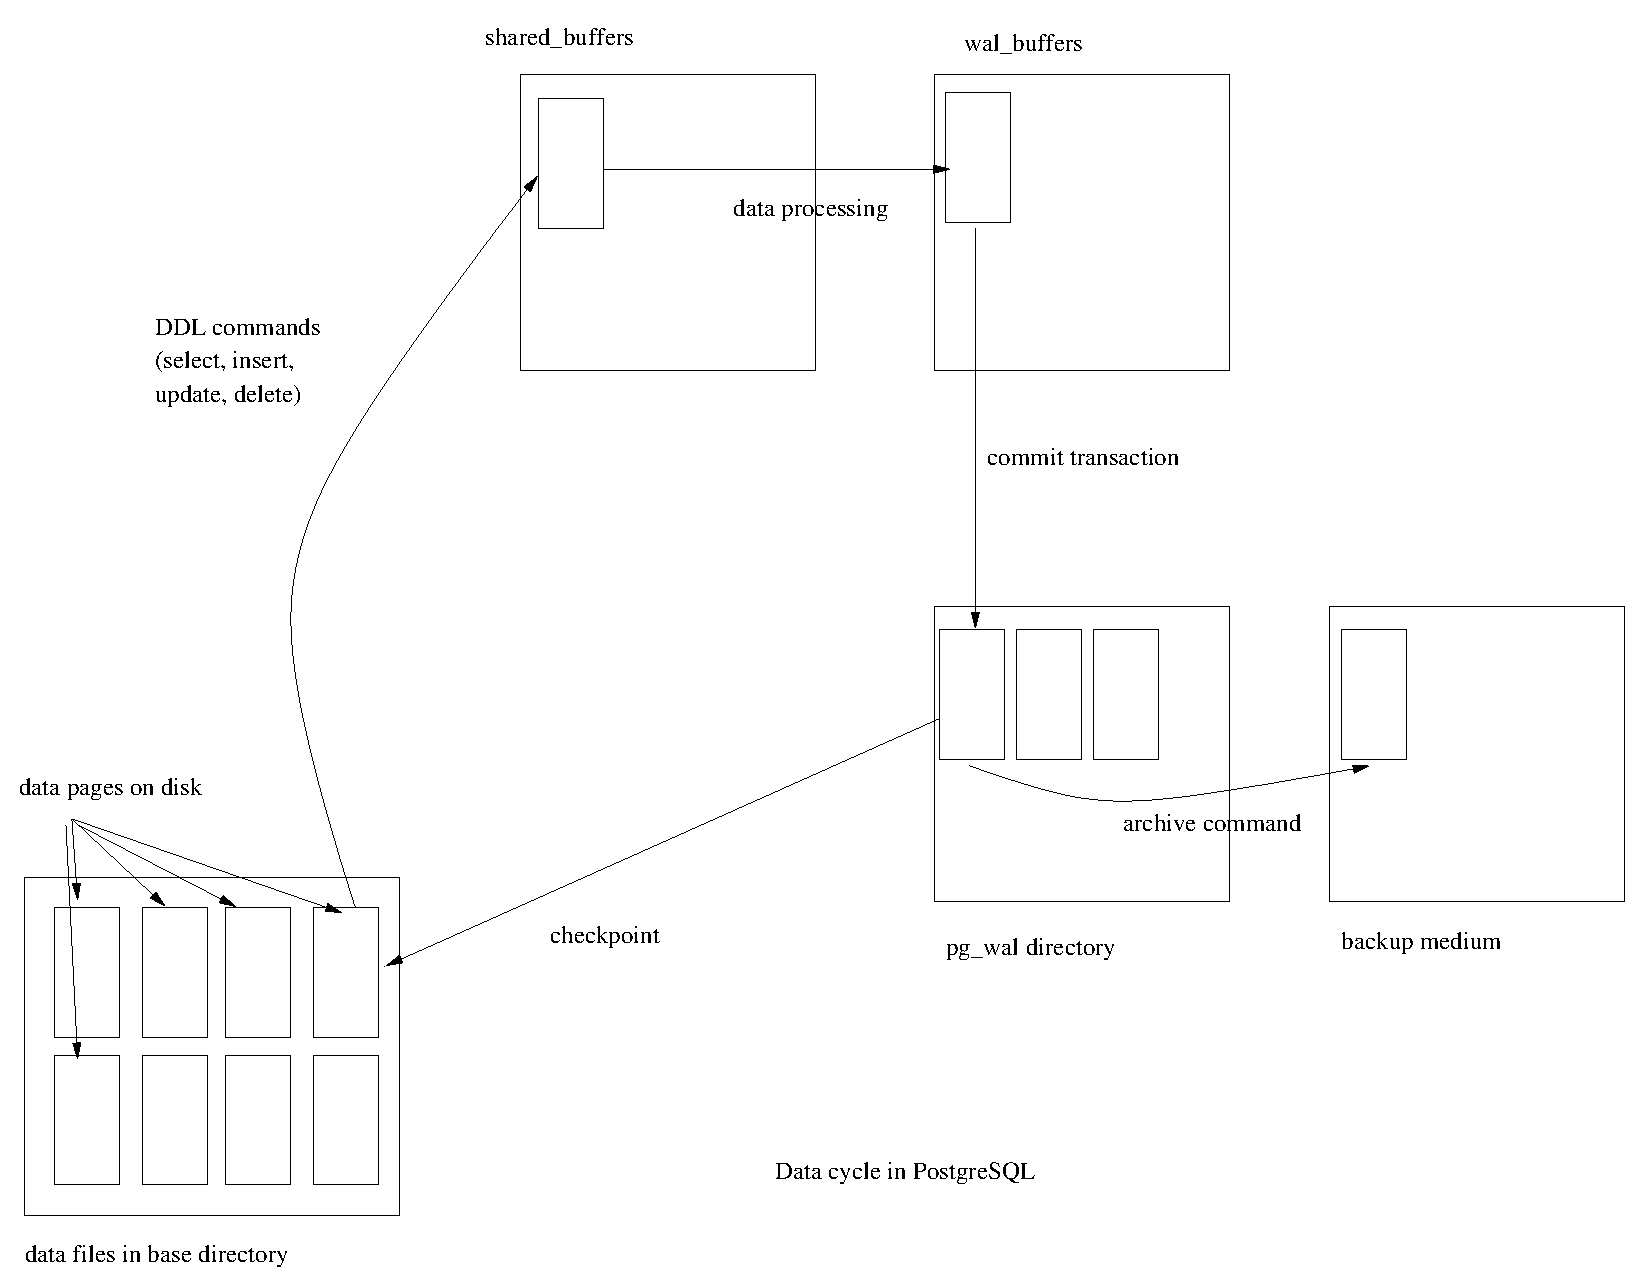
\includegraphics[angle=0, width=0.5\textwidth]{images/internals.eps}
\end{center}
\end{figure}

\begin{toile}
\toileurl{https://www.postgresql.org/docs/15/wal-configuration.html}
\end{toile}

\end{frame}

%%%%%%%%%%%%%%%%%%%%%%%%%%%%%%%%%%%%%%%%%%%%%%%%%%%%%%%%%%%%%%%%%%%%%%%%%%%%%%%%

\begin{frame}{L'importance des sauvegardes}

\begin{itemize}

\item Il est important de posséder 2 copies supplémentaires à la copie des données de productions.
\item Une des 2 copies se situe hors site.
\item Chacune des 2 copies est stockée sur un média différent.

\end{itemize}

\begin{toile}
\toileurl{https://www.it-connect.fr/sauvegarde-quest-ce-que-la-regle-du-3-2-1/}
\end{toile}

\end{frame}

%%%%%%%%%%%%%%%%%%%%%%%%%%%%%%%%%%%%%%%%%%%%%%%%%%%%%%%%%%%%%%%%%%%%%%%%%%%%%%%%

\begin{frame}[fragile]{Différents types de sauvegardes}

Il existe différents types de sauvegarde:

\begin{itemize}

   \item logique avec les commandes \commande{pg\_dump} et \commande{pg\_dumpall}
   \item au niveau du système de fichiers avec la commande \commande{tar}.\footnote{La sauvegarde du système de fichiers n'est pas recommandée par la documentation officielle de PostgreSQL}
   \item binaire avec la commande \commande{pg\_basebackup}

\end{itemize}

\begin{toile}
\toileurl{https://www.postgresql.org/docs/15/backup.html}
\end{toile}

\end{frame}

%%%%%%%%%%%%%%%%%%%%%%%%%%%%%%%%%%%%%%%%%%%%%%%%%%%%%%%%%%%%%%%%%%%%%%%%%%%%%%%%

\begin{frame}[fragile]{Mise en place de la génération des WAL}

\begin{itemize}

   \item Pour activer la génération des WAL, merci de modifier les paramètres suivants dans \textit{postgresql.conf}

\begin{intercom}
wal\_level = replica # or higher
archive\_mode = on
[...]
\end{intercom}

\end{itemize}

\begin{toile}
\toileurl{https://www.postgresql.org/docs/15/continuous-archiving.html}
\end{toile}

\end{frame}

%%%%%%%%%%%%%%%%%%%%%%%%%%%%%%%%%%%%%%%%%%%%%%%%%%%%%%%%%%%%%%%%%%%%%%%%%%%%%%%%

\begin{frame}[fragile]{\commande{archive\_command} et \commande{archive\_library}}

\begin{itemize}

   \item La copie des WAL vers le système de sauvegarde se paramètre depuis les 2 valeurs suivantes:

   \begin{itemize}
      \item \textbf{archive\_command}: Commandes shell d'archivage des WAL
      \item \textbf{archive\_library}: Binaire d'archivage des WAL
   \end{itemize}

   \item Chacune des 2 valeur s'utilise au choix. Elles ne peuvent utilisées en même temps.
   \item Pour les exercices, le paramètre \textbf{archive\_command} sera utilisé.

\begin{scriptsize}
   \begin{intercom}
archive\_command = 'test ! -f /mnt/server/archivedir/\%f && cp \%p /mnt/server/archivedir/\%f' # Unix
   [...]
   \end{intercom}
\end{scriptsize}

\end{itemize}

\end{frame}

%%%%%%%%%%%%%%%%%%%%%%%%%%%%%%%%%%%%%%%%%%%%%%%%%%%%%%%%%%%%%%%%%%%%%%%%%%%%%%%%

\begin{frame}[fragile]{Fonctionnement de l'archivage des WAL}

\begin{itemize}

   \item La commande d'archivage des WALs est lancée par le même utilisateur du process \textit{postmaster}
   \item Elle est censée renvoyer un code différent de 0 en cas d'erreur
   \item Il est important de vérifier que le WAL n'existe pas dans le répertoire cible sous peine de l'écraser
   \item En cas d'erreur d'archivage, PostgreSQL retente autant de fois que nécessaire
   \item Tant que le fichier WAL n'est pas archivé, celui-ci n'est pas supprimé du répertoire pg\_wal, ce qui peut amener à une saturation du système de fichiers
   \item En cas de saturation du répertoire pg\_wal, le serveur s'arrête avec une erreur de type PANIC. Il pourra redémarrer une fois qu'il aura de l'espace disque disponible

\end{itemize}

\end{frame}

%%%%%%%%%%%%%%%%%%%%%%%%%%%%%%%%%%%%%%%%%%%%%%%%%%%%%%%%%%%%%%%%%%%%%%%%%%%%%%%%

\begin{frame}[fragile]{Caractéristique des WAL}

\begin{itemize}

   \item Le nom des fichiers WAL inclut jusqu'à 64 caractères
   \item Il est composé de lettres ASCII, de chiffres et de points
   \item Il est important de garder le nom de l'archive WAL
   \item La sauvegarde des WALs ne permet pas de restaurer \textit{postgresql.conf}, \textit{pg\_hba.conf} ou \textit{pg\_ident.conf}
   \item Il est important de sauvegarder ces 3 fichiers indépendamment
   \item Ces fichiers peuvent être stockés dans un répertoire paramétrable

\end{itemize}

\end{frame}

%%%%%%%%%%%%%%%%%%%%%%%%%%%%%%%%%%%%%%%%%%%%%%%%%%%%%%%%%%%%%%%%%%%%%%%%%%%%%%%%

\begin{frame}[fragile]{La commande \commande{pg\_basebackup}}

\begin{itemize}

\item La commande \commande{pg\_basebackup} sauvegarde un cluster PostgreSQL
\item Elle ne s'applique sur une base de données en particulier
\item L'utilisateur lançant cette commande doit posséder le droit \textbf{REPLICATION} ou être un super-utilisateur
\item La commande peut être lancée sur un serveur standby
\item La table \textit{pg\_stat\_progress\_basebackup} donne une idée de la progression de la commande

\end{itemize}

\begin{toile}
\toileurl{https://www.postgresql.org/docs/15/app-pgbasebackup.html}
\toileurl{https://www.postgresql.org/docs/15/progress-reporting.html\#BASEBACKUP-PROGRESS-REPORTING}
\end{toile}

\end{frame}

%%%%%%%%%%%%%%%%%%%%%%%%%%%%%%%%%%%%%%%%%%%%%%%%%%%%%%%%%%%%%%%%%%%%%%%%%%%%%%%%

\begin{frame}{Options de la commande \commande{pg\_basebackup}}

   Les options qui semblent les plus intéressantes sont:

\begin{itemize}

   \item \option{-F \textit{format}}
   \item \textit{format} a les valeurs suivantes:
   \begin{itemize}
      \item  \textit{p} ou \textit{plain}. Format par défaut. 
      \item  \textit{t} ou \textit{tar}. Génération d'une archive du répertoire des données \textit{base.tar}
   \end{itemize}

\end{itemize}

\begin{toile}
\toileurl{https://www.postgresql.org/docs/15/app-pgbasebackup.html}
\end{toile}

\end{frame}

%%%%%%%%%%%%%%%%%%%%%%%%%%%%%%%%%%%%%%%%%%%%%%%%%%%%%%%%%%%%%%%%%%%%%%%%%%%%%%%%

\begin{frame}{Options de la commande \commande{pg\_basebackup}}

\begin{itemize}
   \item \option{-R} or \option{{-}{-}write-recovery-conf}
   \begin{itemize}
      \item la commande génère automatiquement le fichier \textbf{standby.signal}
   \end{itemize}
   \item \option{-T \textit{olddir}=\textit{newdir}} ou \option{{-}{-}tablespace-mapping=\textit{olddir}=\textit{newdir}}
   \begin{itemize}
      \item cette option permet de mapper les répertoires du serveur liés aux tablespaces à d'autres répertoires locaux. Option valide uniquement si le format \textbf{plain} est utilisé. 
   \end{itemize}
   \item \option{-X \textit{method}} ou \option{{-}{-}wal-method=\textit{method}}
   \begin{itemize}
   \item \textit{method} a les valeurs suivantes:
      \begin{itemize}
         \item  \textit{n} ou \textit{none}. Le backup n'inclut pas les WAL.
         \item  \textit{f} ou \textit{fetch}. Les WAL générés durant le backup sont récupérés une fois le backup généré. Dans le cas de l'utilisation de cette option, le paramètre \option{wal\_keep\_size} nécessite d'être ajusté correctement afin que le serveur puisse garder l'ensemble des WAL (et ne supprime ni n'en recycle durant le backup).
         \item  \textit{s} ou \textit{stream}. Mode par défaut. Une $2^{\grave{e}me}$ connexion est établie vers le serveur pour streamer les WAL générés durant le backup.
      \end{itemize}
   \end{itemize}
\end{itemize}

\end{frame}

%%%%%%%%%%%%%%%%%%%%%%%%%%%%%%%%%%%%%%%%%%%%%%%%%%%%%%%%%%%%%%%%%%%%%%%%%%%%%%%%

\begin{frame}{Options de la commande \commande{pg\_basebackup}}

\begin{itemize}
   \item \option{{-}{-}no-estimate-size}
   \begin{itemize}
      \item le serveur n'estime plus la taille du backup avant de débuter le process. Cela permet de raccourcir la durée de la génération du backup.
   \end{itemize}

\item{\textbf{Environment}}
   \begin{itemize}
      \item Cet utilitaire, tout comme la majorité des utilitaires PostgreSQL, utilisent les mêmes variables d'environnement que ceux de la libpq.
      \item The environment variable PG\_COLOR specifies whether to use color in diagnostic messages. Possible values are \textsl{always}, \textsl{auto} and \textsl{never}.
      \item La variable d'environment PG\_COLOR indique si la couleur est utilisée dans les messages de diagnostique. Les valeurs possibles sont \textsl{always}, \textsl{auto} et \textsl{never}.
   \end{itemize}
\end{itemize}

\end{frame}

%%%%%%%%%%%%%%%%%%%%%%%%%%%%%%%%%%%%%%%%%%%%%%%%%%%%%%%%%%%%%%%%%%%%%%%%%%%%%%%%

\begin{frame}[fragile]{La commande \commande{pg\_verifybackup}}

\begin{itemize}

   \item La commande \commande{pg\_verifybackup} vérifie l'intégrité d'une sauvegarde générée par la commande \commande{pg\_basebackup}

\end{itemize}

\begin{toile}
\toileurl{https://www.postgresql.org/docs/15/app-pgverifybackup.html}
\end{toile}

\end{frame}

%%%%%%%%%%%%%%%%%%%%%%%%%%%%%%%%%%%%%%%%%%%%%%%%%%%%%%%%%%%%%%%%%%%%%%%%%%%%%%%%

\begin{frame}[fragile]{La commande \commande{pg\_amcheck}}

\begin{itemize}

   \item La commande \commande{pg\_amcheck} vérifie l'intégrité d'une base de données.
   \item Fait appel à l'utilitaire \textsf{amcheck}
   \item S'applique aux tables ordinaires, celles de type TOAST, les vues matérialisées, les séquences, les indexes btree.
   \item Possède des options de filtrages de base, de schéma et de table

\end{itemize}

\begin{toile}
\toileurl{https://www.postgresql.org/docs/current/app-pgamcheck.html}
\toileurl{https://www.postgresql.org/docs/current/amcheck.html}
\end{toile}

\end{frame}

%%%%%%%%%%%%%%%%%%%%%%%%%%%%%%%%%%%%%%%%%%%%%%%%%%%%%%%%%%%%%%%%%%%%%%%%%%%%%%%%

\begin{frame}[fragile]{Principales options de la commande \commande{pg\_amcheck}}

   Les principales options de cette commande sont:

\begin{itemize}

   \item \option{{-}{-}no-dependent-indexes} exclut de la vérification les indexes associés à la table
   \item \option{{-}{-}no-dependent-toast} exclut de la vérification les tables TOAST associées à la table
   \item Options applicables aux indexes

   \begin{itemize}
      \item \option{{-}{-}heapallindexed} crée un nouvel index temporaire en mémoire pour vérifier que l'index actuellement stocké est valide. Cette option utilise de la RAM limitée par le paramètre \option{maintenance\_work\_mem}
   \end{itemize}
\end{itemize}

\end{frame}

%%%%%%%%%%%%%%%%%%%%%%%%%%%%%%%%%%%%%%%%%%%%%%%%%%%%%%%%%%%%%%%%%%%%%%%%%%%%%%%%

\begin{frame}{Options de la commande \commande{pg\_amcheck}}

\begin{itemize}
   \item \option{{-}{-}parent-check} vérifie les indexes de la table parent\footnote{https://www.postgresql.org/docs/current/ddl-inherit.html}
\end{itemize}

\end{frame}

%%%%%%%%%%%%%%%%%%%%%%%%%%%%%%%%%%%%%%%%%%%%%%%%%%%%%%%%%%%%%%%%%%%%%%%%%%%%%%%%

\begin{frame}{Réalisation d'un backup de la base de données}

Il existe 2 méthodes pour réaliser une sauvegarde de la base données:
\begin{itemize}
   \item l'outil \textsf{pg\_basebackup}
   \item l'API bas niveau avec des appels aux fonctions PostgreSQL
\end{itemize}

\end{frame}

%%%%%%%%%%%%%%%%%%%%%%%%%%%%%%%%%%%%%%%%%%%%%%%%%%%%%%%%%%%%%%%%%%%%%%%%%%%%%%%%

\begin{frame}{Utilisation de \textsf{pg\_basebackup} pour sauvegarder la base de données}

\begin{itemize}
   \item Vérifier que PostgreSQL est déployé sur le serveur \textsf{hqpg-0x}
   \item Mettre en place la copie des WAL vers le répertoire \path{/opt/wal\_backup} avec le niveau \textsf{replica}
   \item Sur \textsf{hqpg-0x-repl} réaliser une sauvegarde avec la commande \commande{pg\_basebackup}
   \item La commande \textsf{archive\_command} s'appuie sur rsync pour transférer les WALs depuis le primaire. Pour éviter d'avoir à indiquer le mot de l'utilisater postgres, réaliser la génération et l'échange mutuel de clefs SSH sur les 2 serveurs comme décrit en page ~\ref{sec:ssh-keys}


\end{itemize}

\end{frame}

%%%%%%%%%%%%%%%%%%%%%%%%%%%%%%%%%%%%%%%%%%%%%%%%%%%%%%%%%%%%%%%%%%%%%%%%%%%%%%%%

\begin{frame}{Utilisation de \textsf{pg\_basebackup} pour sauvegarder la base de données}

\begin{itemize}
   \item Paramétrer la commande \textsf{archive\_command} dans postgresql.conf
   \begin{itemize}
      \item \commande{archive\_command = 'rsync \%p hqpg-0x-repl:/opt/wal\_backup/\%f'}
   \end{itemize}

   \item Sur le serveur de sauvegarde, créer le répertoire \textsf{/opt/wal\_backup/} de sauvegarde des WALs avec l'utilisateur postgres
\end{itemize}

\end{frame}

%%%%%%%%%%%%%%%%%%%%%%%%%%%%%%%%%%%%%%%%%%%%%%%%%%%%%%%%%%%%%%%%%%%%%%%%%%%%%%%%

\begin{frame}[fragile]\frametitle{Création du jeu de données}

Sur le serveur principal, lancer les commandes suivantes:

\begin{verbatim}
su - postgres
creatuser hq -d
createdb hqdb -O hq
psql hqdb
-- 16h27
create table test\_pitr1 (col1 text);
create table test\_pitr2 (col1 text);
-- quelques minutes plus tard
-- 16h30
create table test\_pitr3 (col1 text);
\end{verbatim}

\begin{toile}
\toileurl{https://www.postgresql.org/docs/current/app-createuser.html}
\toileurl{https://www.postgresql.org/docs/current/app-createdb.html}
\end{toile}


\end{frame}

%%%%%%%%%%%%%%%%%%%%%%%%%%%%%%%%%%%%%%%%%%%%%%%%%%%%%%%%%%%%%%%%%%%%%%%%%%%%%%%%

\begin{frame}[fragile]\frametitle{Utilisation de \textsf{pg\_basebackup} pour sauvegarder la base de données}

Sur le serveur principal, ajouter la ligne suivante dans pg\_hba.conf:

\begin{verbatim}
host    replication     postgres        10.10.10.0/24           trust
\end{verbatim}

Recharger le paramétrage avec la commande suivante:
\begin{verbatim}
postgres=# SELECT pg_reload_conf();
\end{verbatim}

Sur le serveur de sauvegarde des WAL, appliquer les commandes suivantes:

\begin{itemize}
   \item \commande{pg\_basebackup -h hqpg-0x -Ft -z -P -D /opt/backup/20230213}
\end{itemize}

\end{frame}

%%%%%%%%%%%%%%%%%%%%%%%%%%%%%%%%%%%%%%%%%%%%%%%%%%%%%%%%%%%%%%%%%%%%%%%%%%%%%%%%

\begin{frame}[fragile]\frametitle{Inspection de l'archive générée}

\begin{verbatim}
[postgres@localhost 20230202_1]$ ls -lrt
total 4420
-rw------- 1 postgres postgres  181880  2 févr. 07:58 backup_manifest
-rw------- 1 postgres postgres 4321056  2 févr. 07:58 base.tar.gz
-rw------- 1 postgres postgres   17075  2 févr. 07:58 pg_wal.tar.gz
\end{verbatim}

\begin{itemize}
   \item backup\_manifest inclut le listing avec les checkum de l'archive base.tar.gz
   \item pg\_wal.tar.gz inclut les WAL générés durant l'opération du pg\_basebackup
\end{itemize}

\end{frame}

%%%%%%%%%%%%%%%%%%%%%%%%%%%%%%%%%%%%%%%%%%%%%%%%%%%%%%%%%%%%%%%%%%%%%%%%%%%%%%%%

\begin{frame}[fragile]\frametitle{Restauration de la base de données juste avant la création de la table test\_pitr3}

\begin{itemize}
   \item backup\_manifest inclut le listing avec les checkum de l'archive base.tar.gz
   \item pg\_wal.tar.gz inclut les WAL générés durant l'opération du pg\_basebackup
\end{itemize}

\end{frame}

%%%%%%%%%%%%%%%%%%%%%%%%%%%%%%%%%%%%%%%%%%%%%%%%%%%%%%%%%%%%%%%%%%%%%%%%%%%%%%%%

\begin{frame}[fragile]\frametitle{Génération et échange mutuel des clés SSH}
\label{sec:ssh-keys}

\begin{verbatim}
[linagora@localhost ~]$ sudo -i
[root@localhost ~]# su - postgres
[postgres@localhost ~]$ ssh-keygen 
Generating public/private rsa key pair.
Enter file in which to save the key (/var/lib/pgsql/.ssh/id_rsa): 
Enter passphrase (empty for no passphrase): 
Enter same passphrase again: 
\end{verbatim}

\begin{itemize}
   \item Copier la clef publique dans le répertoire $\sim/postgres/.ssh/authorized\_keys$
   \item Vérifier avec la commande ssh \textsf{postgres@hqpg-0x-repl} et inversement que la session SSH est établie sans avoir à fournir de mot de passe
\end{itemize}

\end{frame}

%%%%%%%%%%%%%%%%%%%%%%%%%%%%%%%%%%%%%%%%%%%%%%%%%%%%%%%%%%%%%%%%%%%%%%%%%%%%%%%%

\begin{frame}{Utilisation de \textsf{pg\_basebackup} pour sauvegarder la base de données}

\begin{itemize}
   \item Comme indiqué dans\footnote{https://www.postgresql.org/docs/current/app-pgbasebackup.html}, la commande \textsf{pg\_basebackup} réalise un checkpoint sur le serveur
   \item Les 2 tables précédemment créées sont donc présentes dans la sauvegarde
   \item \commande{pg\_basebackup -h hqpg-0x -Ft -z -P -D /usr/local/pgsql/data}
\end{itemize}

\end{frame}

%%%%%%%%%%%%%%%%%%%%%%%%%%%%%%%%%%%%%%%%%%%%%%%%%%%%%%%%%%%%%%%%%%%%%%%%%%%%%%%%

\begin{frame}[fragile]{Supervision de la base de données}

   TODO

\begin{itemize}

   \item TODO

\end{itemize}

\begin{toile}
\toileurl{https://www.postgresql.org/docs/15/monitoring.html}
\end{toile}

\end{frame}

%%%%%%%%%%%%%%%%%%%%%%%%%%%%%%%%%%%%%%%%%%%%%%%%%%%%%%%%%%%%%%%%%%%%%%%%%%%%%%%%

\begin{frame}[fragile]{En cas de corruption des WALs}

\begin{itemize}

   \item If recovery finds corrupted WAL data, recovery will halt at that point and the server will not start. In such a case the recovery process could be re-run from the beginning, specifying a “recovery target” before the point of corruption so that recovery can complete normally.    \item If recovery fails for an external reason, such as a system crash or if the WAL archive has become inaccessible, then the recovery can simply be restarted and it will restart almost from where it failed. 
   \item Recovery restart works much like checkpointing in normal operation: the server periodically forces all its state to disk, and then updates the pg\_control file to indicate that the already-processed WAL data need not be scanned again.

\end{itemize}

\begin{toile}
\toileurl{https://www.postgresql.org/docs/15/continuous-archiving.html}
\end{toile}

\end{frame}


%%%%%%%%%%%%%%%%%%%%%%%%%%%%%%%%%%%%%%%%%%%%%%%%%%%%%%%%%%%%%%%%%%%%%%%%%%%%%%%%

\newlength{\largeurtableau}
\setlength{\largeurtableau}{\textwidth}
\addtolength{\largeurtableau}{-2\leftmarginii}

%%%%%%%%%%%%%%%%%%%%%%%%%%%%%%%%%%%%%%%%%%%%%%%%%%%%%%%%%%%%%%%%%%%%%%%%%%%%%%%%

\begin{frame}{\path{/proc}}

\begin{itemize}

\item Le pseudo-système de fichiers \path{/proc} contient :

	\begin{itemize}

	\item un répertoire par processus, nommé selon son PID

	\item un lien symbolique \path{self} pointant vers le répertoire
	correspondant au processus courant

	\item divers fichiers contenant des informations générales, par
	exemple :

\bigskip

\begin{tabulary}{\largeurtableau}{lJ}
\hline
\path{/proc/cmdline}	& paramètres passés au noyau par le chargeur
				d'amorçage		\\
\path{/proc/cpuinfo}	& microprocesseur(s)		\\
\path{/proc/interrupts}	& interruptions			\\
\path{/proc/loadavg}	& charge moyenne		\\
\path{/proc/meminfo}	& utilisation de la mémoire	\\
\hline
\end{tabulary}

	\end{itemize}

\end{itemize}

\begin{toile}
\toileurl{http://fr.wikipedia.org/wiki/Procfs}
\end{toile}

\end{frame}

%%%%%%%%%%%%%%%%%%%%%%%%%%%%%%%%%%%%%%%%%%%%%%%%%%%%%%%%%%%%%%%%%%%%%%%%%%%%%%%%

\begin{frame}[fragile]{\path{/sys}}

\begin{itemize}

\item Le pseudo-système de fichiers \path{/sys} fournit de nombreuses
informations concernant le matériel et les pilotes.

\item Exemple :

\begin{intercom}
\$ cat /sys/class/net/eth0/address
00:1c:23:30:20:13
\end{intercom}

\end{itemize}

\begin{toile}
\toileurl{http://fr.wikipedia.org/wiki/Sysfs}
\end{toile}

\end{frame}

%%%%%%%%%%%%%%%%%%%%%%%%%%%%%%%%%%%%%%%%%%%%%%%%%%%%%%%%%%%%%%%%%%%%%%%%%%%%%%%%

\subsection{Démarrage du système}

%%%%%%%%%%%%%%%%%%%%%%%%%%%%%%%%%%%%%%%%%%%%%%%%%%%%%%%%%%%%%%%%%%%%%%%%%%%%%%%%

% TODO démarrage single user

%%%%%%%%%%%%%%%%%%%%%%%%%%%%%%%%%%%%%%%%%%%%%%%%%%%%%%%%%%%%%%%%%%%%%%%%%%%%%%%%

% TODO Provide common commands to the boot loader and options to the kernel at boot time.
% TODO Demonstrate knowledge of the boot sequence from BIOS to boot completion.
% TODO Check boot events in the log files.

% TODO /var/log/messages

%%%%%%%%%%%%%%%%%%%%%%%%%%%%%%%%%%%%%%%%%%%%%%%%%%%%%%%%%%%%%%%%%%%%%%%%%%%%%%%%

\subsection{Changement de niveaux d'exécution et arrêt ou redémarrage du système}

%%%%%%%%%%%%%%%%%%%%%%%%%%%%%%%%%%%%%%%%%%%%%%%%%%%%%%%%%%%%%%%%%%%%%%%%%%%%%%%%

\begin{frame}{Les commandes \commande{halt}, \commande{poweroff} et
\commande{reboot}}

\begin{itemize}

\item Équivalentes à la commande \commande{shutdown} utilisée avec certaines
options :

\bigskip

\begin{tabular}{|l|l|}
\hline
\commande{halt}		& \commande{shutdown} \option{-H}	\\
\hline
\commande{poweroff}	& \commande{shutdown} \option{-P}	\\
\hline
\commande{reboot}	& \commande{shutdown} \option{-r}	\\
\hline
\end{tabular}

\bigskip

\item Contrairement à \commande{shutdown}, ces commandes ne permettent
d'indiquer ni de délai (elles ont un effet immédiat) ni de message pour les
utilisateurs connectés.

\end{itemize}

\begin{toile}
\toileurl{http://fr.wikipedia.org/wiki/Halt}
\end{toile}

\end{frame}

%%%%%%%%%%%%%%%%%%%%%%%%%%%%%%%%%%%%%%%%%%%%%%%%%%%%%%%%%%%%%%%%%%%%%%%%%%%%%%%%

% TODO Knowledge of basic features of systemd and Upstart.

\include{pitr/pitr.tex}
%%%%%%%%%%%%%%%%%%%%%%%%%%%%%%%%%%%%%%%%%%%%%%%%%%%%%%%%%%%%%%%%%%%%%%%%%%%%%%%%

\section{Supervision du serveur de base de données}

%%%%%%%%%%%%%%%%%%%%%%%%%%%%%%%%%%%%%%%%%%%%%%%%%%%%%%%%%%%%%%%%%%%%%%%%%%%%%%%%

\begin{frame}[fragile]{Supervision de la base de données}

   TODO
   WIP

\begin{toile}
\toileurl{https://www.postgresql.org/docs/15/monitoring.html}
\end{toile}

\end{frame}

%%%%%%%%%%%%%%%%%%%%%%%%%%%%%%%%%%%%%%%%%%%%%%%%%%%%%%%%%%%%%%%%%%%%%%%%%%%%%%%%

\begin{frame}{Supervision de l'activité des disques}

\begin{itemize}

   \item TODO

\end{itemize}

\begin{toile}
\toileurl{https://www.postgresql.org/docs/15/diskusage.html}
\end{toile}

\end{frame}

%%%%%%%%%%%%%%%%%%%%%%%%%%%%%%%%%%%%%%%%%%%%%%%%%%%%%%%%%%%%%%%%%%%%%%%%%%%%%%%%


% TODO Knowledge of basic features of systemd and Upstart.


%%%%%%%%%%%%%%%%%%%%%%%%%%%%%%%%%%%%%%%%%%%%%%%%%%%%%%%%%%%%%%%%%%%%%%%%%%%%%%%%

\begin{frame}{L'examen 101}

\begin{itemize}

\item Dure 1 h 30.

\item Comprend 60 questions.

\item Le score maximum est de 800.

\item Un score de 500 est nécessaire pour réussir l'examen.

\item C'est-à-dire 62,5 \% du score maximum soit environ 37,5 questions.

\end{itemize}

\begin{toile}
\toileurl{http://www.lpi.org/linux-certifications/programs/lpic-1/exam-101/}
\toileurl{http://wiki.lpi.org/wiki/LPIC-1_Objectives(FR)\#Objectifs_de_l.27examen_LPI_101}
\end{toile}

\end{frame}

%%%%%%%%%%%%%%%%%%%%%%%%%%%%%%%%%%%%%%%%%%%%%%%%%%%%%%%%%%%%%%%%%%%%%%%%%%%%%%%%

\section*{Bibliographie}

\pdfbookmark[2]{Bibliographie}{bibliographie}

%%%%%%%%%%%%%%%%%%%%%%%%%%%%%%%%%%%%%%%%%%%%%%%%%%%%%%%%%%%%%%%%%%%%%%%%%%%%%%%%

\section*{Webographie}

\pdfbookmark[2]{Webographie}{webographie}


%%%%%%%%%%%%%%%%%%%%%%%%%%%%%%%%%%%%%%%%%%%%%%%%%%%%%%%%%%%%%%%%%%%%%%%%%%%%%%%%


%%%%%%%%%%%%%%%%%%%%%%%%%%%%%%%%%%%%%%%%%%%%%%%%%%%%%%%%%%%%%%%%%%%%%%%%%%%%%%%%

\section*{Sommaire}

\pdfbookmark[2]{Sommaire}{sommaire}

\begin{frame}{Sommaire}

\tableofcontents[hideallsubsections]

\end{frame}

%%%%%%%%%%%%%%%%%%%%%%%%%%%%%%%%%%%%%%%%%%%%%%%%%%%%%%%%%%%%%%%%%%%%%%%%%%%%%%%%

\section*{Conclusion}

\pdfbookmark[2]{Conclusion}{conclusion}

%\merci

%%%%%%%%%%%%%%%%%%%%%%%%%%%%%%%%%%%%%%%%%%%%%%%%%%%%%%%%%%%%%%%%%%%%%%%%%%%%%%%%

\end{document}
